\documentclass[dvipdfmx,cjk,10.2pt]{beamer} 
%\documentclass[dvipdfm,cjk]{beamer} %% オプションは環境や利用するプログラムに
%\documentclass[dvips,cjk]{beamer}   %% よって変える

\usepackage{tikz}
\usepackage{subfigure}
\usepackage[all]{xy}
\usepackage{wrapfig}

\newcommand{\R}{\mathbb{R}}
\newcommand{\Q}{\mathbb{Q}}
\newcommand{\Z}{\mathbb{Z}}
\newcommand{\N}{\mathbb{N}}



\makeatletter
\newcommand\xleftrightarrow[2][]{%
  \ext@arrow 9999{\longleftrightarrowfill@}{#1}{#2}}
\newcommand\longleftrightarrowfill@{%
  \arrowfill@\leftarrow\relbar\rightarrow}
\makeatother

\AtBeginDvi{\special{pdf:tounicode 90ms-RKSJ-UCS2}} %% しおりが文字化けしないように
%\AtBeginDvi{\special{pdf:tounicode EUC-UCS2}}

\setbeamertemplate{navigation symbols}{} %% 右下のアイコンを消す
\setbeamertemplate{theorems}[normal font] %%斜体を直す

\usetheme{CambridgeUS}         %% theme の選択
%\usetheme{Boadilla}           %% Beamer のディレクトリの中の
%\usetheme{Madrid}             %% beamerthemeCambridgeUS.sty を指定
%\usetheme{Antibes}            %% 色々と試してみるといいだろう
%\usetheme{Montpellier}        %% サンプルが beamer\doc に色々とある。
%\usetheme{Berkeley}
%\usetheme{Goettingen}
%\usetheme{Singapore}
%\usetheme{Szeged}

%\usecolortheme{rose}          %% colortheme を選ぶと色使いが変わる
%\usecolortheme{albatross}

%\useoutertheme{shadow}                 %% 箱に影をつける
\usefonttheme{professionalfonts}       %% 数式の文字を通常の LaTeX と同じにする

%\setbeamercovered{transparent}         %% 消えている文字をうっすらと表示する


\theoremstyle{definition}
\setbeamertemplate{theorems}[numbered]  %% 定理に番号をつける
\newtheorem{Thm}{定理}[section]
%\theoremstyle{example}
\newtheorem{Ex}[Thm]{例}
%\newtheorem{exam}[thm]{Example}
\newtheorem{Rem}[Thm]{注意}
\newtheorem{Conj}[Thm]{予想}
\newtheorem{Def}[Thm]{定義}
\newtheorem{Prob}[Thm]{問題}

\setbeamercolor{block title}{fg=blue!70!black, bg=blue!15!white} 
\setbeamercolor{block body}{fg=black, bg=blue!10!white}



\begin{document}
\title{微分・積分 第9回} 
\author{慶応義塾大学}            %% ここに書かれた情報は色々なところに使われるので
\institute[]{総合政策学部・環境情報学部}   %% なるべく設定した方が良い
\date{}



\begin{frame}                  %% \begin{frame}..\end{frame} で 1 枚のスライド
\titlepage                     %% タイトルページ
\end{frame}

%\begin{frame}                  %% 目次 (必要なければ省略)
%\tableofcontents
%\end{frame}






%%%%%%%%%%%%%%%%%%%%%%%%%%%%%%%%%%%%%%%%%%%%%%%%%%%%%%%%%%%%%%%%%%%%%%%%%%%%%%%%%%%%%%%
%%%%%%%%%%%%%%%%%%%%%%%%%%%%%%%%%%%%%%%%%%%%%%%%%%%%%%%%%%%%%%%%%%%%%%%%%%%%%%%%%%%%%%%

\section{講義概要}


\begin{frame}
\frametitle{今日の内容}


前回に引き続いてテイラーの定理に関する話題を議論する. 
\begin{enumerate}
\item テイラーの定理の証明
\item テイラー展開, 解析的関数
\item 応用, オイラーの公式
\end{enumerate} 



\end{frame}




%%%%%%%%%%%%%%%%%%%%%%%%%%%%%%%%%%%%%%%%%%%%%%%%%%%%%%%%%%%%%%%%%%%%%%%%%%%%%%%%%%%%%%%
%%%%%%%%%%%%%%%%%%%%%%%%%%%%%%%%%%%%%%%%%%%%%%%%%%%%%%%%%%%%%%%%%%%%%%%%%%%%%%%%%%%%%%%


%%%%%%%%%%%%%%%%%%%%%%%%%%%%%%%%%%%%%%%%%%%%%%%%%%%%%%%%%%%%%%%%%%%%%%%%%%%%%%%%%%%%%%%
%%%%%%%%%%%%%%%%%%%%%%%%%%%%%%%%%%%%%%%%%%%%%%%%%%%%%%%%%%%%%%%%%%%%%%%%%%%%%%%%%%%%%%%

\section{テイラーの定理}

\begin{frame}
\frametitle{関数の多項式近似}


\begin{itemize}
\item 微分とは, 関数を$1$次多項式(関数)で近似した様子を記述するもの. 
導関数の情報から関数の増減の解析が可能になった. 
\item 導関数がさらに微分可能ならば, $2$回微分することにより凹凸を知ることができた. 
これは関数を$2$次多項式で近似することに相当する.
\item 関数がさらに微分可能の場合には, $3$回微分, $4$回微分, ... を考えることにより, 
与えられた関数の$3$次多項式, $4$次多項式, ... で近似できる. 
\end{itemize}
一般の関数(三角関数, 指数関数, 対数関数)などは難しいが, 多項式関数は比較的簡単である. 

\end{frame}




%%%%%%%%%%%%%%%%%%%%%%%%%%%%%%%%%%%%%%%%%%%%%%%%%%%%%%%%%%%%%%%%%%%%%%%%%%%%%%%%%%%%%%%
%%%%%%%%%%%%%%%%%%%%%%%%%%%%%%%%%%%%%%%%%%%%%%%%%%%%%%%%%%%%%%%%%%%%%%%%%%%%%%%%%%%%%%%




\begin{frame}
\frametitle{テイラーの定理}

\begin{Thm}[テイラーの定理] \label{テイラー}
開区間$I$で定義された関数$f(x)$が$n$回微分可能であるとき. 
任意の$a \in I$に対して, 
 \begin{align*}
f(x) & = \sum_{k=0}^{n-1}\frac{f^{(k)}(a)}{k!}(x-a)^k + \frac{f^{(n)}(c)}{k!}(x-a)^n \\
& =  f(a)+ f'(a)(x-a) + \frac{f^{(2)}(a)}{2!}(x-a)^2  + \frac{f^{(3)}(a)}{3!}(x-a)^3 \\
& \ \ \ + \dots + \frac{f^{(n-1)}(a)}{(n-1)!}(x-a)^{n-1}+\frac{f^{(n)}(c)}{k!}(x-a)^n . 
\end{align*}
を満たす$c \in (a,x)$が存在する. ($a<x$の場合) 
\end{Thm}
上記の表示を有限テイラー展開という.

\end{frame}





%%%%%%%%%%%%%%%%%%%%%%%%%%%%%%%%%%%%%%%%%%%%%%%%%%%%%%%%%%%%%%%%%%%%%%%%%%%%%%%%%%%%%%%
%%%%%%%%%%%%%%%%%%%%%%%%%%%%%%%%%%%%%%%%%%%%%%%%%%%%%%%%%%%%%%%%%%%%%%%%%%%%%%%%%%%%%%%



\begin{frame}
\frametitle{マクローリンの定理}


特に$a=0$の場合にはマクローリンの定理と呼ばれる. 


\begin{Thm}[マクローリンの定理]  \label{マクローリン}
$0$を含む開区間$I$で定義された関数$f(x)$が$n$回微分可能であるとき. 
 \begin{align*}
f(x) & = \sum_{k=0}^{n-1}\frac{f^{(k)}(0)}{k!}x^k + \frac{f^{(n)}(\theta x)}{n!}x^n \\
& =  f(0)+ f'(0)x + \frac{f^{(2)}(0)}{2!}x^2  + \frac{f^{(3)}(0)}{3!}x^3 \\
& \ \ \ + \dots + \frac{f^{(n-1)}(0)}{(n-1)!}x^{n-1}+\frac{f^{(n)}(\theta x)}{n!}x^n . 
\end{align*}
を満たす$\theta \in (0,1)$が存在する. ($0<x$の場合) 
\end{Thm}
$\theta x \in (0,x)$に注意. 上記の表示を有限マクローリン展開という.

\end{frame}


%%%%%%%%%%%%%%%%%%%%%%%%%%%%%%%%%%%%%%%%%%%%%%%%%%%%%%%%%%%%%%%%%%%%%%%%%%%%%%%%%%%%%%%
%%%%%%%%%%%%%%%%%%%%%%%%%%%%%%%%%%%%%%%%%%%%%%%%%%%%%%%%%%%%%%%%%%%%%%%%%%%%%%%%%%%%%%%


%%%%%%%%%%%%%%%%%%%%%%%%%%%%%%%%%%%%%%%%%%%%%%%%%%%%%%%%%%%%%%%%%%%%%%%%%%%%%%%%%%%%%%%
%%%%%%%%%%%%%%%%%%%%%%%%%%%%%%%%%%%%%%%%%%%%%%%%%%%%%%%%%%%%%%%%%%%%%%%%%%%%%%%%%%%%%%%



\begin{frame}
\frametitle{テイラーの定理}


\begin{itemize}
\item テイラーの定理における
$$
P_{n-1}(x)=\sum_{k=0}^{n-1}\frac{f^{(k)}(a)}{k!}(x-a)^k, \ \ \ 
R_n(x)=\frac{f^{(n)}(c)}{k!}(x-a)^n
$$
はそれぞれ($n-1$次の)\underline{テイラー多項式}と\underline{剰余項}と呼ばれる. 
\item 微分の観点からは, $f(x)$と$P_{n-1}(x)$は似ている. 
$$
f(a)=P_{n-1}(a), \ \ f '(a)=P'_{n-1}(a), \ \dots, \  f^{(n-1)}(a)=P^{(n-1)}_{n-1}(a). 
$$
実際, $f(x)$が$n$次多項式であれば, $f(x)=P_n(x)$であった. 
\item テイラーの定理は$f(x)$と$P_{n-1}(x)$の誤差を$f(x)$の$n$次微分係数を用いて評価できることを主張している. 
\end{itemize}

\end{frame}



%%%%%%%%%%%%%%%%%%%%%%%%%%%%%%%%%%%%%%%%%%%%%%%%%%%%%%%%%%%%%%%%%%%%%%%%%%%%%%%%%%%%%%%
%%%%%%%%%%%%%%%%%%%%%%%%%%%%%%%%%%%%%%%%%%%%%%%%%%%%%%%%%%%%%%%%%%%%%%%%%%%%%%%%%%%%%%%





\begin{frame}
\frametitle{$e^x$の有限マクローリン展開}

$f(x)=e^x$の有限マクローリン展開
\begin{align*}
e^x &= P_5(x)+R_6(x) \\
& = 1+x+\frac{x^2}{2!}+\frac{x^3}{3!}+\frac{x^4}{4!}+\frac{x^5}{5!}+\frac{e^{\theta x}}{6!}x^6. 
\end{align*}
を用いて$f(1)=e$の近似値を求める. 
$$
P_5(1)=\frac{163}{60}=2.71666\dots
$$
であるが, テイラーの定理より誤差は
$$
|e-P_5(1)|=\frac{e^\theta}{6!}<\frac{e}{6!}<\frac{3}{6!}=\frac{1}{240}=0.004166\dots
$$

\end{frame}




%%%%%%%%%%%%%%%%%%%%%%%%%%%%%%%%%%%%%%%%%%%%%%%%%%%%%%%%%%%%%%%%%%%%%%%%%%%%%%%%%%%%%%%
%%%%%%%%%%%%%%%%%%%%%%%%%%%%%%%%%%%%%%%%%%%%%%%%%%%%%%%%%%%%%%%%%%%%%%%%%%%%%%%%%%%%%%%


\section{テイラーの定理の証明}

\begin{frame}
\frametitle{コーシーの平均値の定理}

コーシーの平均値の定理を用いて, テイラーの定理を証明する. 

\begin{Thm}[コーシーの平均値の定理] 
微分可能な関数$f(x)$, $g(x)$の定義域に$[a,b]$が含まれ, $a<x<b$において$g'(x) \ne 0$であれば, 
$$
\frac{f(b)-f(a)}{g(b)-g(a)}=\frac{f'(c)}{g'(c)}
$$
なる$c \in (a,b)$が存在する. 
\end{Thm}

直感的には媒介変数$t \in [a,b]$を用いて$(x,y)=(g(t),f(t))$の軌跡を考えれば良い. 

\vspace{-5mm}

 \begin{figure}[htbp]
 \begin{center} 
  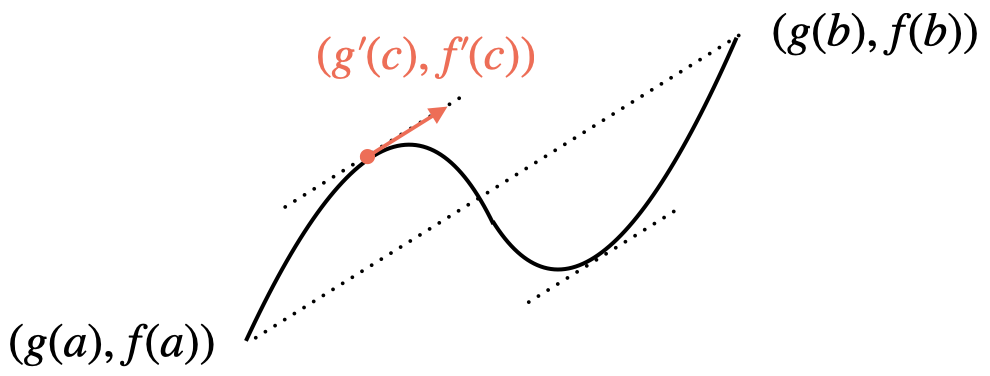
\includegraphics[width=55mm]{CauchyMean.png}
 \end{center}
\end{figure}

\end{frame}




%%%%%%%%%%%%%%%%%%%%%%%%%%%%%%%%%%%%%%%%%%%%%%%%%%%%%%%%%%%%%%%%%%%%%%%%%%%%%%%%%%%%%%%
%%%%%%%%%%%%%%%%%%%%%%%%%%%%%%%%%%%%%%%%%%%%%%%%%%%%%%%%%%%%%%%%%%%%%%%%%%%%%%%%%%%%%%%


\section{テイラーの定理の証明}

\begin{frame}
\frametitle{テイラーの定理の証明}

関数 \vspace{-5mm}
\begin{align*}
 F(x) =&  f(x)-\sum_{k=0}^{n-1}\frac{f^{(k)}(a)}{k!}(x-a)^k \\
=&   f(x)-\big\{ f(a)+ f'(a)(x-a) + \frac{f^{(2)}(a)}{2!}(x-a)^2   \\
& \ \ \ + \dots + \frac{f^{(n-1)}(a)}{(n-1)!}(x-a)^{n-1}\big\}
\end{align*}
を考え, これが剰余項$\frac{f^{(n)}(c)}{n!}(x-a)^n \ (a<c<x)$の形に書けることを示す. 
簡単な計算で次が分かる. 
\begin{itemize}
\item $F(a)=F'(a)=F''(a)= \dots =F^{(n-1)}(a)=0$, 
\item $F^{(n)}(a)=f^{(n)}(a)$. 
\end{itemize}  

\end{frame}


%%%%%%%%%%%%%%%%%%%%%%%%%%%%%%%%%%%%%%%%%%%%%%%%%%%%%%%%%%%%%%%%%%%%%%%%%%%%%%%%%%%%%%%
%%%%%%%%%%%%%%%%%%%%%%%%%%%%%%%%%%%%%%%%%%%%%%%%%%%%%%%%%%%%%%%%%%%%%%%%%%%%%%%%%%%%%%%



\begin{frame}
\frametitle{テイラーの定理の証明}

\begin{itemize}
\item $F(x)$と$G(x)=(x-a)^n$に対して, コーシーの平均値の定理を使うと
\begin{align*}
\frac{F(x)}{G(x)}=\frac{F(x)-F(a)}{G(x)-G(a)}=\frac{F'(x_1)}{G'(x_1)}
\end{align*}
なる$a<x_1<x$が存在する. 
\item $F'(x)$と$G'(x)=n(x-a)^{n-1}$に対して, コーシーの平均値の定理を使うと
\begin{align*}
\frac{F'(x_1)}{G'(x_1)}=\frac{F'(x_1)-F'(a)}{G'(x_1)-G'(a)}=\frac{F''(x_2)}{G''(x_2)}
\end{align*}
なる$a<x_2<x_1$が存在する. 
\item これを繰り返す. 
\end{itemize}
\end{frame}


%%%%%%%%%%%%%%%%%%%%%%%%%%%%%%%%%%%%%%%%%%%%%%%%%%%%%%%%%%%%%%%%%%%%%%%%%%%%%%%%%%%%%%%
%%%%%%%%%%%%%%%%%%%%%%%%%%%%%%%%%%%%%%%%%%%%%%%%%%%%%%%%%%%%%%%%%%%%%%%%%%%%%%%%%%%%%%%



\begin{frame}
\frametitle{テイラーの定理の証明}

纏めると
\begin{align*}
\frac{F(x)}{G(x)}=\frac{F'(x_1)}{G'(x_1)}
=\frac{F''(x_2)}{G''(x_2)}=\dots =\frac{F^{(n-1)}(x_{n-1})}{G^{(n-1)}(x_{n-1})}=\frac{F^{(n)}(x_{n})}{G^{(n)}(x_{n})}
\end{align*}
なる$a<x_{n}<x_{n-1}<\dots<x_1<x$が存在する. 
これより
$$
\frac{F(x)}{(x-a)^n}=\frac{F(x)}{G(x)}=\frac{F^{(n)}(x_{n})}{G^{(n)}(x_{n})}=\frac{f^{(n)}(x_n)}{n!}
$$
なので, $c=x_n$として
$$
F(x)=\frac{f^{(n)}(c)}{n!}(x-a)^n
$$
が示された. 

\end{frame}



%%%%%%%%%%%%%%%%%%%%%%%%%%%%%%%%%%%%%%%%%%%%%%%%%%%%%%%%%%%%%%%%%%%%%%%%%%%%%%%%%%%%%%%
%%%%%%%%%%%%%%%%%%%%%%%%%%%%%%%%%%%%%%%%%%%%%%%%%%%%%%%%%%%%%%%%%%%%%%%%%%%%%%%%%%%%%%%


\section{テイラー展開}

\begin{frame}
\frametitle{テイラー展開}


\begin{itemize}
%\item テイラーの定理とマクローリンの定理で得られるの関数の表示をそれぞれ有限テイラー展開, 有限マクローリン展開という. 
\item $C^\infty$級関数$f(x)$に関して
剰余項
$$
R_n=\frac{f^{(n)}(c)}{k!}(x-a)^n \rightarrow 0 \ \ \ (n \rightarrow \infty)
$$
が成立すれば, $f(x)$は冪級数展開(単項式の無限和として表現)
$$
f(x) = \sum_{k=0}^{\infty}\frac{f^{(k)}(a)}{k!}(x-a)^k. 
$$
としての表示を持つ.  
\item 剰余項$R_n$に関する条件は, $x$が$a$に十分近いときに満たされることが多いが, この講義では深入りしない. (収束半径の議論が必要.)
\end{itemize}

\end{frame}


%%%%%%%%%%%%%%%%%%%%%%%%%%%%%%%%%%%%%%%%%%%%%%%%%%%%%%%%%%%%%%%%%%%%%%%%%%%%%%%%%%%%%%%
%%%%%%%%%%%%%%%%%%%%%%%%%%%%%%%%%%%%%%%%%%%%%%%%%%%%%%%%%%%%%%%%%%%%%%%%%%%%%%%%%%%%%%%



\begin{frame}
\frametitle{テイラー展開}

\begin{Def}
$C^\infty$級関数$f(x)$に関して, 剰余項が$R_n \to 0$ $(n \rightarrow \infty)$なるとき
\begin{align*}
f(x) & = \sum_{k=0}^{\infty}\frac{f^{(k)}(a)}{k!}(x-a)^k \\
& =  f(a)+ f'(a)(x-a) + \frac{f^{(2)}(a)}{2!}(x-a)^2  + \frac{f^{(3)}(a)}{3!}(x-a)^3 \\
& \ \ \ + \dots + \frac{f^{(n)}(a)}{n!}(x-a)^{n}+\dots. 
\end{align*}
この表示を$f(x)$の\underline{テイラー展開}と呼ぶ. 
特に$a=0$のときは, マクローリン展開と呼ばれる. 
\end{Def}

\end{frame}



%%%%%%%%%%%%%%%%%%%%%%%%%%%%%%%%%%%%%%%%%%%%%%%%%%%%%%%%%%%%%%%%%%%%%%%%%%%%%%%%%%%%%%%
%%%%%%%%%%%%%%%%%%%%%%%%%%%%%%%%%%%%%%%%%%%%%%%%%%%%%%%%%%%%%%%%%%%%%%%%%%%%%%%%%%%%%%%



\begin{frame}
\frametitle{$e^x$のマクローリン展開}

$f(x)=e^x$に関して, $f^{(n)}(x)=e^x$であるから, 有限マクローリン展開は
$$
e^x=1+x+\frac{x^2}{2!}+\frac{x^3}{3!}+\dots+\frac{x^{n-1}}{(n-1)!}+\frac{e^{\theta x}}{n!}x^n. 
$$
ただし$0<\theta < 1$. 
任意の$x$に対して
$$
\frac{e^{\theta x}}{n!}x^n \to 0 \ \ \ (n \to \infty)
$$
であるから, $f(x)=e^x$のマクローリン展開は
$$
e^x= \sum_{k=0}^{\infty}\frac{x^k}{k!}
=1+x+\frac{x^2}{2!}+\frac{x^3}{3!}+\dots
$$
簡単のため, $0<x$としたが, $0>x$でも成立する.  
\end{frame}



%%%%%%%%%%%%%%%%%%%%%%%%%%%%%%%%%%%%%%%%%%%%%%%%%%%%%%%%%%%%%%%%%%%%%%%%%%%%%%%%%%%%%%%
%%%%%%%%%%%%%%%%%%%%%%%%%%%%%%%%%%%%%%%%%%%%%%%%%%%%%%%%%%%%%%%%%%%%%%%%%%%%%%%%%%%%%%%



\begin{frame}
\frametitle{$\sin x$のマクローリン展開}

$f(x)=\sin x$の有限マクローリン展開を求める. 
$$
f'(x)=\cos x, \ f^{(2)}(x)=-\sin x, \ f^{(3)}(x)=-\cos x, \ f^{(4)}(x)=\sin x
$$
を周期$4$で繰り返すことから
$$
 f^{(4n)}(0)=0, \ f^{(4n+1)}(0)=1, \ f^{(4n+2)}(0)=0, \ f^{(4n+3)}(0)=-1. 
$$
したがって
\begin{align*}
\sin x & = \sum_{k=0}^{n-1}(-1)^k\frac{x^{2k+1}}{(2k+1)!}+R \\
& = x-\frac{x^3}{3!}+\frac{x^5}{5!}+\dots+\frac{(-1)^{n-1}}{(2n-1)!}x^{2n-1}+R
\end{align*}
	

\end{frame}




%%%%%%%%%%%%%%%%%%%%%%%%%%%%%%%%%%%%%%%%%%%%%%%%%%%%%%%%%%%%%%%%%%%%%%%%%%%%%%%%%%%%%%%
%%%%%%%%%%%%%%%%%%%%%%%%%%%%%%%%%%%%%%%%%%%%%%%%%%%%%%%%%%%%%%%%%%%%%%%%%%%%%%%%%%%%%%%



\begin{frame}
\frametitle{$\sin x$のマクローリン展開}

ただし, 剰余項$R$は$R_{2n}$または$R_{2n+1}$であり, ある$0 < \theta <1$に関して
$$
R_{2n}=\frac{(-1)^n \sin(\theta x)}{(2n)!}x^{2n}, \ \ \ R_{2n+1}=\frac{(-1)^n \cos(\theta x)}{(2n+1)!}x^{2n+1}. 
$$
いずれの場合も
$$
|R_N| \le \frac{x^N}{N!} \to 0 \ \ \ (N \to \infty) 
$$
であるから, $f(x)=\sin x$のマクローリン展開は
\begin{align*}
\sin x & = \sum_{k=0}^{\infty}(-1)^k\frac{x^{2k+1}}{(2k+1)!} \\
& = x-\frac{x^3}{3!}+\frac{x^5}{5!}-\frac{x^7}{7!}+\dots 
\end{align*}

\end{frame}


%%%%%%%%%%%%%%%%%%%%%%%%%%%%%%%%%%%%%%%%%%%%%%%%%%%%%%%%%%%%%%%%%%%%%%%%%%%%%%%%%%%%%%%
%%%%%%%%%%%%%%%%%%%%%%%%%%%%%%%%%%%%%%%%%%%%%%%%%%%%%%%%%%%%%%%%%%%%%%%%%%%%%%%%%%%%%%%



\begin{frame}
\frametitle{$\cos x$のマクローリン展開}

$f(x)=\cos x$のマクローリン展開も同様に求めることができる. 

\begin{align*}
\cos x & = \sum_{k=0}^{\infty}(-1)^k\frac{x^{2k}}{(2k)!} \\
& = 1-\frac{x^2}{2!}+\frac{x^4}{4!}-\frac{x^6}{6!}+\dots 
\end{align*}

これらのマクローリン展開からも, $(\sin x)'=\cos x$, $(\cos x)' = -\sin x$が成立していることが分かる. (項別微分)

\end{frame}


%%%%%%%%%%%%%%%%%%%%%%%%%%%%%%%%%%%%%%%%%%%%%%%%%%%%%%%%%%%%%%%%%%%%%%%%%%%%%%%%%%%%%%%
%%%%%%%%%%%%%%%%%%%%%%%%%%%%%%%%%%%%%%%%%%%%%%%%%%%%%%%%%%%%%%%%%%%%%%%%%%%%%%%%%%%%%%%



\begin{frame}
\frametitle{三角関数と弧度法}

解析学において, 三角関数を弧度法で考えることは重要である. 
実際, 度数法の世界では三角関数の基本的な公式は複雑になる($1^\circ=\frac{\pi}{180}$rad):  
\begin{itemize}
\item $\displaystyle \lim_{x\to0}\frac{\sin x}{x}=\frac{\pi}{180}$
\item $\displaystyle (\sin x)'=\frac{\pi}{180} \cos x, \ \ \  (\cos x)'=-\frac{\pi}{180} \sin x$
\item $\displaystyle \sin x = \frac{\pi}{180} x - \frac{\pi^3}{180^3}\frac{x^3}{3!}+\frac{\pi^5}{180^5}\frac{x^5}{5!}+\dots$
\end{itemize}
弧度法では形式的にラジアンという単位を使うが, 実際は円の半径と弧の比であるから(長さの単位に依存しない)無次元量である. 
本来, 数は無次元量であり, それゆえ$x+x^3$のような計算が意味を持つのである. 

\end{frame}


%%%%%%%%%%%%%%%%%%%%%%%%%%%%%%%%%%%%%%%%%%%%%%%%%%%%%%%%%%%%%%%%%%%%%%%%%%%%%%%%%%%%%%%
%%%%%%%%%%%%%%%%%%%%%%%%%%%%%%%%%%%%%%%%%%%%%%%%%%%%%%%%%%%%%%%%%%%%%%%%%%%%%%%%%%%%%%%



\begin{frame}
\frametitle{$\frac{1}{1-x}$のマクローリン展開}

$f(x)=\frac{1}{1-x}$の有限マクローリン展開を求める. 
\begin{align*}
f'(x)=\frac{1}{(1-x)^2}, \ \ \ f''(x)=\frac{2}{(1-x)^3}, \ \ \  f^{(3)}(x)=\frac{3\cdot 2}{(1-x)^4}, \dots 
\end{align*}
であり, 一般に$f^{(k)}(x)=\frac{k!}{(1-x)^{k+1}}$であるから
\begin{align*}
\frac{1}{1-x} & = \sum_{k=0}^{n-1}x^k+\frac{1}{(1-\theta x)^{n+1}}x^n \\
& = 1+x+x^2+\dots+x^{n-1}+\frac{1}{(1-\theta x)^{n+1}}x^n
\end{align*}
ただし$0<\theta < 1$. 

\end{frame}

%%%%%%%%%%%%%%%%%%%%%%%%%%%%%%%%%%%%%%%%%%%%%%%%%%%%%%%%%%%%%%%%%%%%%%%%%%%%%%%%%%%%%%%
%%%%%%%%%%%%%%%%%%%%%%%%%%%%%%%%%%%%%%%%%%%%%%%%%%%%%%%%%%%%%%%%%%%%%%%%%%%%%%%%%%%%%%%



\begin{frame}
\frametitle{$\frac{1}{1-x}$のマクローリン展開}

$0\le x<1/2$であれば
$$
\frac{|x|^n}{|1-\theta x|^{n+1}} \le \frac{|x|^n}{|1-|x||^{n+1}} \to 0 \ \ \ (n\to \infty)
$$
であるから, $\frac{1}{1-x}$のマクローリン展開は
\begin{align*}
\frac{1}{1-x} & = \sum_{k=0}^{\infty} x^k \\
&=1+x+x^2+x^3+x^4+\dots. 
\end{align*}
実際には, $-1<x<1$においてマクローリン展開が成立する. 
(等比数列の和と思えば良い.)

\end{frame}



%%%%%%%%%%%%%%%%%%%%%%%%%%%%%%%%%%%%%%%%%%%%%%%%%%%%%%%%%%%%%%%%%%%%%%%%%%%%%%%%%%%%%%%
%%%%%%%%%%%%%%%%%%%%%%%%%%%%%%%%%%%%%%%%%%%%%%%%%%%%%%%%%%%%%%%%%%%%%%%%%%%%%%%%%%%%%%%



\begin{frame}
\frametitle{$\log(1+x)$のマクローリン展開}

$f(x)=\log(1+x)$の有限マクローリン展開を求める. 
\begin{align*}
f'(x)=\frac{1}{1+x}, \ \ \  f''(x)=\frac{-1}{(1+x)^2}, \ \ \  f^{(2)}(x)=\frac{2}{(1+x)^3}, \dots
\end{align*}
であり, 一般に$f^{(k)}(x)=\frac{(-1)^{k+1}(k-1)!}{(1+x)^{k}}$であるから
\begin{align*}
\log(1+x) &= \sum_{k=1}^{n-1}(-1)^{k+1}\frac{x^k}{k}+\frac{(-1)^{n+1}}{n(1+\theta x)^{n}}x^n \\
& = x-\frac{x^2}{2}+\frac{x^3}{3}+ \dots +(-1)^{n}\frac{x^{n-1}}{n-1}+\frac{(-1)^{n+1}}{n(1+\theta x)^{n}}x^n. 
\end{align*}
ただし$0<\theta < 1$. 

\end{frame}




%%%%%%%%%%%%%%%%%%%%%%%%%%%%%%%%%%%%%%%%%%%%%%%%%%%%%%%%%%%%%%%%%%%%%%%%%%%%%%%%%%%%%%%
%%%%%%%%%%%%%%%%%%%%%%%%%%%%%%%%%%%%%%%%%%%%%%%%%%%%%%%%%%%%%%%%%%%%%%%%%%%%%%%%%%%%%%%


\begin{frame}
\frametitle{$\log(1+x)$のマクローリン展開}

$0\le x\le 1$であれば
$$
\frac{|(-1)^{n+1}x^n|}{|n(1+\theta x)^{n}|} \le \frac{1}{n} \to 0 \ \ \ (n\to \infty)
$$
であるから, $\log(1+x)$のマクローリン展開は
\begin{align*}
\log(1+x) & =  \sum_{k=1}^{\infty}(-1)^{k+1}\frac{x^k}{k} \\
& =  x-\frac{x^2}{2}+\frac{x^3}{3} - \frac{x^4}{4}+\dots.
\end{align*}
実際は, $-1<x<1$においてマクローリン展開が成立する. 

\end{frame}

%%%%%%%%%%%%%%%%%%%%%%%%%%%%%%%%%%%%%%%%%%%%%%%%%%%%%%%%%%%%%%%%%%%%%%%%%%%%%%%%%%%%%%%
%%%%%%%%%%%%%%%%%%%%%%%%%%%%%%%%%%%%%%%%%%%%%%%%%%%%%%%%%%%%%%%%%%%%%%%%%%%%%%%%%%%%%%%


\section{解析関数}

\begin{frame}
\frametitle{解析関数}

\begin{Def}
$C^\infty$級関数$f(x)$が$a$の近傍で, テイラー展開
$$
f(x) = \sum_{k=0}^{\infty}\frac{f^{(k)}(a)}{k!}(x-a)^k 
$$
されるとき, $f(x)$は$a$で\underline{解析的}と呼ばれる. 定義域の任意の点で解析的な関数を\underline{解析的関数}という. 
\end{Def}

\end{frame}


%%%%%%%%%%%%%%%%%%%%%%%%%%%%%%%%%%%%%%%%%%%%%%%%%%%%%%%%%%%%%%%%%%%%%%%%%%%%%%%%%%%%%%%
%%%%%%%%%%%%%%%%%%%%%%%%%%%%%%%%%%%%%%%%%%%%%%%%%%%%%%%%%%%%%%%%%%%%%%%%%%%%%%%%%%%%%%%



\begin{frame}
\frametitle{解析的でない$C^\infty$関数}


$C^\infty$関数であっても, 解析的でない関数は存在する. 例えば
$$
f(x) = 
\begin{cases}
e^{-\frac{1}{x}}  & (x>0) \\
0 & (x \le 0) 
 \end{cases}
$$
原点$0$において解析的でない. \\
\ \\

実際, 
$$
f'(x)=\frac{1}{x^2}e^{-\frac{1}{x}} \longrightarrow 0 \ \ \ (x \to +0)
$$
といった計算から, 全ての$n \in \N$に対し$f^{(n)}(0)=0$が成立している. 
もし$f(x)$がマクローリン展開可能とすると, $f(x)=0$となって矛盾する. 
\end{frame}




%%%%%%%%%%%%%%%%%%%%%%%%%%%%%%%%%%%%%%%%%%%%%%%%%%%%%%%%%%%%%%%%%%%%%%%%%%%%%%%%%%%%%%%
%%%%%%%%%%%%%%%%%%%%%%%%%%%%%%%%%%%%%%%%%%%%%%%%%%%%%%%%%%%%%%%%%%%%%%%%%%%%%%%%%%%%%%%

\section{応用}

\begin{frame}
\frametitle{$\sin 1$の近似値}

$\sin x$のマクローリン展開 
$$
\sin x = x-\frac{x^3}{3!}+\frac{x^5}{5!}-\frac{x^7}{7!}+\frac{x^9}{9!}+\dots 
$$
を用いて, $\sin 1$の近似値を求める. 
\begin{align*}
& 1-\frac{1^3}{3!}+\frac{1^5}{5!} = \frac{101}{120}=0.84166\dots \\
& 1-\frac{1^3}{3!}+\frac{1^5}{5!}-\frac{1^7}{7!} = \frac{4241}{5040}=0.841468\dots \\
& 1-\frac{1^3}{3!}+\frac{1^5}{5!}-\frac{1^7}{7!}+\frac{1^9}{9!} = \frac{305353}{362880}=0.841471\dots
\end{align*}
実際, $\sin 1 = 0.841470\dots$. 
\end{frame}






%%%%%%%%%%%%%%%%%%%%%%%%%%%%%%%%%%%%%%%%%%%%%%%%%%%%%%%%%%%%%%%%%%%%%%%%%%%%%%%%%%%%%%%
%%%%%%%%%%%%%%%%%%%%%%%%%%%%%%%%%%%%%%%%%%%%%%%%%%%%%%%%%%%%%%%%%%%%%%%%%%%%%%%%%%%%%%%


\begin{frame}
\frametitle{極限の計算}

\vspace{-5mm}

\begin{align*}
\lim_{x \to 0} \frac{\sin x -x}{x^3} & = \lim_{x \to 0} \frac{(x -\frac{x^3}{3!}+\frac{x^5}{5!}+\dots) -x}{x^3} \\
& =   \lim_{x \to 0} \frac{-\frac{x^3}{6}+\frac{x^5}{120}+\dots}{x^3} \\
& =   \lim_{x \to 0} (-\frac{1}{6}+\frac{x^2}{120}+\dots ) = -\frac{1}{6}. 
\end{align*}

\begin{align*}
\lim_{x \to 0} \frac{e^x-1-x}{x^2} &=  \lim_{x \to 0} \frac{(1+x+\frac{x^2}{2}+\frac{x^3}{6}+\dots )-1-x}{x^2} \\
& = \lim_{x \to 0} \frac{\frac{x^2}{2}+\frac{x^3}{6}+\dots}{x^2} \\
& = \lim_{x \to 0} (\frac{1}{2}+\frac{x}{6}+\dots)= \frac{1}{2}.  
\end{align*}

\end{frame}




%%%%%%%%%%%%%%%%%%%%%%%%%%%%%%%%%%%%%%%%%%%%%%%%%%%%%%%%%%%%%%%%%%%%%%%%%%%%%%%%%%%%%%%
%%%%%%%%%%%%%%%%%%%%%%%%%%%%%%%%%%%%%%%%%%%%%%%%%%%%%%%%%%%%%%%%%%%%%%%%%%%%%%%%%%%%%%%

\section{オイラーの公式}

\begin{frame}
\frametitle{オイラーの公式 (発展)}

指数関数と三角関数は一見無関係のように思えるが, テイラー展開を考えると類似性が浮かび上がってくる. 

\begin{align*}
e^x & = 1+x+\frac{x^2}{2!}+\frac{x^3}{3!}+\frac{x^4}{4!}+\frac{x^5}{5!}+\frac{x^6}{6!}+\frac{x^7}{7!}\dots \\
\sin x &=   \hspace{6.5mm} x  \hspace{9.5mm}   -\frac{x^3}{3!}  \hspace{9.5mm} +\frac{x^5}{5!} \hspace{9.5mm} -\frac{x^7}{7!} +  \dots  \\
\cos x &= 1   \hspace{6.5mm}  -\frac{x^2}{2!}   \hspace{9.5mm} +\frac{x^4}{4!}   \hspace{9.5mm} -\frac{x^6}{6!} +\dots 
\end{align*}

\end{frame}


%%%%%%%%%%%%%%%%%%%%%%%%%%%%%%%%%%%%%%%%%%%%%%%%%%%%%%%%%%%%%%%%%%%%%%%%%%%%%%%%%%%%%%%
%%%%%%%%%%%%%%%%%%%%%%%%%%%%%%%%%%%%%%%%%%%%%%%%%%%%%%%%%%%%%%%%%%%%%%%%%%%%%%%%%%%%%%%

\begin{frame}
\frametitle{オイラーの公式 (発展)}

$i^2=-1$なる虚数 $i$を考えて, 指数関数のテイラー展開において, $x$を$ix$に置き換える. 
\begin{align*}
e^{ix} & = 1+ix+\frac{(ix)^2}{2!}+\frac{(ix)^3}{3!}+\frac{(ix)^4}{4!}+\frac{(ix)^5}{5!}+\frac{(ix)^6}{6!}+\frac{(ix)^7}{7!}+\dots \\
& = 1+ix-\frac{x^2}{2!}-i\frac{x^3}{3!}+\frac{x^4}{4!}+i\frac{x^5}{5!}-\frac{x^6}{6!}-i\frac{x^7}{7!}+\dots \\
& = 1  -\frac{x^2}{2!}  +\frac{x^4}{4!}  -\frac{x^6}{6!} +\dots + i(x  -\frac{x^3}{3!}  +\frac{x^5}{5!} -\frac{x^7}{7!} + \dots ) \\
& = \cos x + i \sin x. 
\end{align*}

$e^{ix}$が何を意味するのかを理解するには, 複素関数論を勉強する必要がある. 

\end{frame}



%%%%%%%%%%%%%%%%%%%%%%%%%%%%%%%%%%%%%%%%%%%%%%%%%%%%%%%%%%%%%%%%%%%%%%%%%%%%%%%%%%%%%%%
%%%%%%%%%%%%%%%%%%%%%%%%%%%%%%%%%%%%%%%%%%%%%%%%%%%%%%%%%%%%%%%%%%%%%%%%%%%%%%%%%%%%%%%


\begin{frame}
\frametitle{オイラーの公式 (発展)}

\begin{Thm}[オイラーの公式]
\begin{center}
$
e^{ix} = \cos x + i \sin x
$
\end{center}
\end{Thm}

特に$x=\pi$とした
$$
e^{i \pi }=-1
$$
は美しい数式として有名である. 


 \begin{figure}[htbp]
 \begin{center} 
  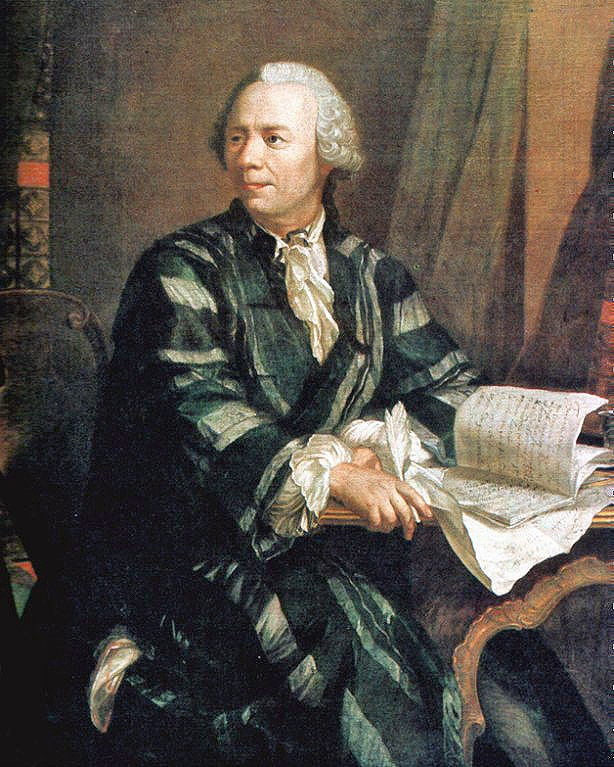
\includegraphics[width=30mm, bb=0 0 614 767]{Euler.jpg}
 \end{center}
\end{figure}

\end{frame}



%%%%%%%%%%%%%%%%%%%%%%%%%%%%%%%%%%%%%%%%%%%%%%%%%%%%%%%%%%%%%%%%%%%%%%%%%%%%%%%%%%%%%%%
%%%%%%%%%%%%%%%%%%%%%%%%%%%%%%%%%%%%%%%%%%%%%%%%%%%%%%%%%%%%%%%%%%%%%%%%%%%%%%%%%%%%%%%






%%%%%%%%%%%%%%%%%%%%%%%%%%%%%%%%%%%%%%%%%%%%%%%%%%%%%%%%%%%%%%%%%%%%%%%%%%%%%%%%%%%%%%%
%%%%%%%%%%%%%%%%%%%%%%%%%%%%%%%%%%%%%%%%%%%%%%%%%%%%%%%%%%%%%%%%%%%%%%%%%%%%%%%%%%%%%%%





%%%%%%%%%%%%%%%%%%%%%%%%%%%%%%%%%%%%%%%%%%%%%%%%%%%%%%%%%%%%%%%%%%%%%%%%%%%%%%%%%%%%%%%
%%%%%%%%%%%%%%%%%%%%%%%%%%%%%%%%%%%%%%%%%%%%%%%%%%%%%%%%%%%%%%%%%%%%%%%%%%%%%%%%%%%%%%%




\section{今日のまとめ}
\begin{frame}
\frametitle{まとめ}   


\begin{enumerate}
\item テイラーの定理の証明
\item テイラー展開, 解析的関数
\item 応用, オイラーの公式
\end{enumerate} 

\end{frame}


\end{document}